\documentclass[10pt]{article}
\usepackage[polish]{babel}
\usepackage[utf8]{inputenc}
\usepackage[T1]{fontenc}
\usepackage{amsmath}
\usepackage{amsfonts}
\usepackage{amssymb}
\usepackage[version=4]{mhchem}
\usepackage{stmaryrd}
\usepackage{graphicx}
\usepackage[export]{adjustbox}
\graphicspath{ {./images/} }

\title{KLASY PIERWSZE I DRUGIE }

\author{}
\date{}


\newcommand\Varangle{\mathop{{<\!\!\!\!\!\text{\small)}}\:}\nolimits}

\begin{document}
\maketitle
\begin{enumerate}
  \item Na okręgu umieszczono 2021 punktów białych i 1 punkt czerwony. Rozpatrujemy wszystkie możliwe wielokąty o wierzchołkach w tych punktach. Których wielokątów jest więcej: mających czerwony wierzchołek, czy mających tylko białe wierzchołki? Odpowiedź uzasadnij.
  \item Boki prostokąta mają długości 10 i 24. Przekątną podzielono ten prostokąt na dwa trójkąty. Oblicz odległość środków okręgów wpisanych w te trójkąty.
  \item Do dwóch okręgów stycznych zewnętrznie w punkcie \(A\) poprowadzono wspólną styczną \(B C\) (punkty \(B\) i \(C\) są punktami styczności). Udowodnij, że odcinki \(A B\) i \(A C\) są prostopadłe.\\
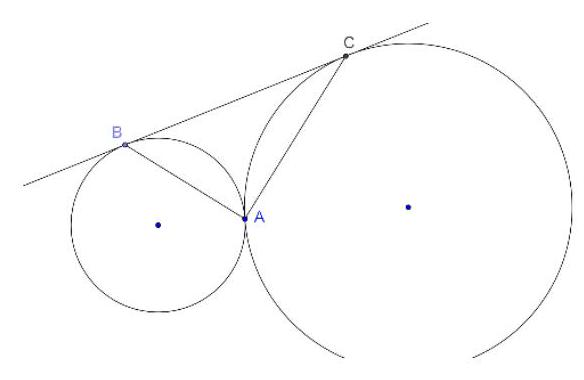
\includegraphics[max width=\textwidth, center]{2024_11_21_4d4a36e74ff5475f5b63g-1}
\end{enumerate}

\section*{KLASY TRZECIE}
\begin{enumerate}
  \item Czworokąt wypukły \(A B C D\) jest wpisany w okrąg. Jego przekątne przecinają się w punkcie E, a kąt BEC jest kątem rozwartym. Prosta przechodząca przez punkt C i prostopadła do prostej AC przecina prostą przechodzącą przez punkt B i prostopadła do prostej BD w punkcie F. Wykaż, że proste EF i AD są prostopadłe.
  \item Niech [XYZ] oznacza pole trójkąta XYZ. W czworokącie wypukłym ABCD zachodzi \(\Varangle D A B+\Varangle A B C=90^{\circ}\), a punkt M jest środkiem boku CD. Znając długości boków AD i BC, które wynoszą odpowiednio \(a\) i \(b\), obliczyć wartość [ABM]-[DAM]-[BCM].
  \item Dany jest trójkąt \(A B C\), w którym \(B C=10, C A=8\). Punkt \(M\) jest środkiem boku \(A B\). Udowodnij, że istnieje dokładnie jeden punkt leżący na okręgu o środku w punkcie M i promieniu 1 dla którego \(\Varangle A X C=90^{\circ}\)
\end{enumerate}

\end{document}